\documentclass[5p,authoryear]{elsarticle}
\makeatletter
\def\ps@pprintTitle{%
 \let\@oddhead\@empty
 \let\@evenhead\@empty
 \let\@evenfoot\@oddfoot} % Supprimer le bas de page ELSEVIER
\makeatother
\usepackage[utf8]{inputenc} % En unicode
\usepackage[T1]{fontenc}
\usepackage{amsmath} % pour certains signes mathématiques
\usepackage{mathtools, amsmath, amsthm, amssymb, amsfonts, physics}
\usepackage{booktabs} % pour \toprule (un style de tableau)
\usepackage{multirow} % Pour colonnes multiples des tableaux
\usepackage{float}
%\usepackage{hyperref} % DOIT ETRE EN DERNIER
\usepackage[scaled]{helvet}
\usepackage{caption}
\usepackage{tikz}
\usepackage{longtable}
\usetikzlibrary{shapes.geometric, arrows, positioning, angles, quotes}
\usetikzlibrary{decorations.pathmorphing}\usepackage{hyphenat}
\usepackage{multicol}
\usetikzlibrary{angles, quotes}
\renewcommand\familydefault{\sfdefault}
\mathtoolsset{showonlyrefs}

\usepackage{xcolor}
\usepackage{color}
% The following special color definitions are used in the IST Thesis
\definecolor{forestgreen}{RGB}{34,139,34}
\definecolor{orangered}{RGB}{239,134,64}
\definecolor{lightred}{rgb}{1,0.4,0.5}
\definecolor{orange}{rgb}{1,0.45,0.13}
\definecolor{darkblue}{rgb}{0.0,0.0,0.6}
\definecolor{lightblue}{rgb}{0.1,0.57,0.7}
\definecolor{gray}{rgb}{0.4,0.4,0.4}
\definecolor{lightgray}{rgb}{0.95, 0.95, 0.95}
\definecolor{darkgray}{rgb}{0.4, 0.4, 0.4}
\definecolor{editorGray}{rgb}{0.95, 0.95, 0.95}
\definecolor{editorOcher}{rgb}{1, 0.5, 0} % #FF7F00 -> rgb(239, 169, 0)
\definecolor{chaptergrey}{rgb}{0.6,0.6,0.6}
\definecolor{editorGreen}{rgb}{0, 0.5, 0} % #007C00 -> rgb(0, 124, 0)
\definecolor{olive}{rgb}{0.17,0.59,0.20}
\definecolor{brown}{rgb}{0.69,0.31,0.31}
\definecolor{purple}{rgb}{0.38,0.18,0.81}

\usepackage{hyperref}
% pre-configuration of hyperref
\hypersetup{ colorlinks=true,
             citecolor=cyan,
             linkcolor=darkgray,
             urlcolor=teal,
             breaklinks=true,
             bookmarksnumbered=true,
             bookmarksopen=true,
}

\newtheorem{theorem}{Theorem}[subsection]
\newtheorem{remark}[theorem]{Remark}
\newtheorem{corollary}[theorem]{Corollary}
\newtheorem{proposition}[theorem]{Proposition}
\newtheorem{lemma}[theorem]{Lemma}
\newtheorem{definition}[theorem]{Definition}
\newtheorem{conjecture}[theorem]{Conjecture}
\newtheorem{example}[theorem]{Example}

\DeclareMathOperator{\Span}{span}
\DeclareMathOperator{\dom}{Dom}
\DeclareMathOperator\supp{supp}
\DeclareMathOperator\Div{div}
\DeclareMathOperator{\atantwo}{atan \mspace{2mu} 2}

% * <mael65@gmail.com> 2015-04-23T12:54:33.332Z:
%
%  Le rapport d'intégration est là : https://www.overleaf.com/2598017ffjjqg
%
% ^ <mael65@gmail.com> 2015-04-25T11:36:30.135Z:
%
%  La présentation là : https://www.overleaf.com/2606987svydrv
%

%\bibliographystyle{elsarticle-num}
\bibliographystyle{alpha}

\begin{document}

\begin{frontmatter}

\title{A numerical study of the Dirac Spectrum and Transmission Problems employing the Method of Fundamental Solutions}

%% Group authors per affiliation:

\author{Francisco Bento \\ \small{\vspace{0.2cm} Supervisors: \\ \vspace{0.1cm} Juha Hans Videman \\ Pedro Ricardo Simão Antunes}}

%\author{}
\address{Instituto Superior Técnico - Lisboa, Portugal}

\begin{abstract}
This dissertation studies the application of the Method of Fundamental Solutions (MFS), a meshless technique, to address a duo of Partial Differential Equations (PDEs) problems. Meshless methods provide an alternative to the standard mesh-based approaches, especially suited for intricate geometries. This study is centered on two focal points: firstly, the spectral analysis of the Dirac operator with infinite mass boundary conditions, investigated through large-scale simulations; secondly, the resolution of transmission problems involving the Poisson equation within polygonal and curved domains.

Within the MFS framework, the spectral behavior of the Dirac operator is explored, both verifying existing conjectures and postulating new ones. The study also covers transmission problems with the Poisson equation, utilizing singularity subtraction techniques to improve the accuracy of the method.

This thesis starts by establishing the necessary theory, rigorously introducing and implementing the MFS, and incorporating strategies to address inherent limitations. The results presented underscore the method's validity in addressing challenging PDE problems, showcasing the effectiveness of meshless methods.
\end{abstract}

\begin{keyword}
    Meshless methods \sep Method of Fundamental Solutions \sep Dirac operator \sep Transmission problems \sep Numerical simulations \sep Singularity subtraction techniques
\end{keyword}

\end{frontmatter}

This work focuses on the Method of Fundamental Solutions (MFS), a meshless technique to solve Partial Differential Equations (PDEs), exploring its applications in the spectral analysis of the Dirac operator under infinite mass boundary conditions and transmission problems involving the Poisson equation in complex domains.

Meshless methods, like the MFS, offer mesh-free alternatives to traditional approaches, avoiding complex mesh generation. The MFS approximates the solution of a PDE using its fundamental solution and has been very effective in solving eigenvalue problems. This study aims to explore its broader applicability for various PDE challenges.

This research goes into the spectral behavior of the Dirac operator under infinite mass boundary conditions, a recent challenge in shape optimization theory. It aims to gain insights into this operator's behavior using the MFS for numerical validation and the generation of new conjectures. Exploring domain decomposition problems with transmission conditions for the Poisson equation, which can be used to model heat conduction and electromagnetism, this study enhances the MFS for polygonal and curved domains, addressing its inherent limitations in less regular domains.

\section{Shape Optimization and the Dirac Operator}

% One of the most classical and well-known problems in shape optimization theory involves the Laplace operator with Dirichlet boundary conditions,

% \begin{equation}\label{helm_equation}
% 	\begin{cases}
% 		-\Delta u = \lambda u, & \text{in } \Omega\\
% 		u = 0, & \text{on } \partial\Omega,
% 	\end{cases}
% \end{equation}
% throughoutly studied in \cite{henrot2006extremum} and \cite{henrot2017shape}, and the determination of optimal shapes for its eigenvalues \(\lambda \in \mathbb{C}\) when subject to various geometric constraints.

% This equation, known as the Helmholtz equation, arises in various areas of physics and engineering and is related to wave propagation, diffusion, and acoustic phenomena. For example, in acoustics, this equation represents the vibration of a membrane with clamped edges, such as a drum. In quantum mechanics, understanding its behavior is fundamental in studying the Schrödinger equation and the energy states of a non-relativistic particle.

% One of the seminal conjectures in shape optimization is the celebrated Faber-Krahn inequality, which was firstly conjectured by Lord Rayleigh at the end of the 19th century and it was later proved in 1923 and 1925 by Faber and Krahn. This inequality posits that among all domains with a fixed volume in Euclidean space, the ball has the smallest first Dirichlet eigenvalue for the Laplace operator.

% \begin{theorem}[Faber-Krahn inequality]\label{faber-krahn}
%     Let \(B \subset \mathbb{R}^d\) be a ball of volume \(c\). Then, among all domains \(\Omega \subset \mathbb{R}^d\) of volume \(c\), we have that
%     \[
%     \lambda_1(B) = \min\{\lambda_1(\Omega): \abs{\Omega} = c\}.
%     \]
% \end{theorem}

% This result has profound implications for understanding the optimal shapes of objects in various mathematical and physical contexts, including minimizing the fundamental vibrational frequency of a drumhead with a fixed area. While various results have been uncovered for the Laplace operator, generalizing the problem \eqref{helm_equation} for different boundary conditions and specific domain types, results concerning high-order eigenvalues are still open.

% In the last decades, due to recent advancements in nuclear, and molecular physics and the discovery of interesting electrical, mechanical, and thermal properties of Dirac materials, a lot of attention has been put on the Dirac equation which generalizes the Schrödinger equation for relativistic particles.

Shape optimization theory has a rich history, with classical emphasis on problems involving the Laplace operator under Dirichlet boundary conditions
\begin{equation}\label{helm_equation}
	\begin{cases}
		-\Delta u = \lambda u, & \text{in } \Omega\\
		u = 0, & \text{on } \partial\Omega,
	\end{cases}
\end{equation}
throughoutly studied in \cite{henrot2006extremum}, and the determination of optimal shapes for its eigenvalues \(\lambda \in \mathbb{R}\) when subject to various geometric constraints. The Laplace operator arises in various fields, from acoustics to quantum mechanics, and determining optimal shapes for its eigenvalues is a fundamental challenge.

One notable result in shape optimization is the Faber-Krahn inequality, which establishes that among domains with fixed volume in Euclidean space, the ball possesses the smallest first Dirichlet eigenvalue for the Laplace operator. However, extending these findings to higher-order eigenvalues remains an open challenge. In recent years, increased attention has been given to the Dirac operator, which generalizes the Schrödinger equation for relativistic particles. This shift in focus is driven by advancements in nuclear and molecular physics and the unique properties of Dirac materials, such as graphene.

% In summary, shape optimization has evolved from its classical roots in Laplace operator problems to encompass broader applications in fields like quantum mechanics, thanks to the relevance of the Dirac operator in modern physics.

Consider an open connected set \(\Omega \subset \mathbb{R}^2\) with Lipschitz boundary \(\Gamma\), a relativistic particle of mass \(m \geq 0\) and the Hamiltonian (Dirac) operator \(\hat{H}\) in \(L^2(\Omega, \mathbb{C}^2)\),
\begin{equation*}
	\hat{H} = \begin{bmatrix}
		m & -i(\partial_1 - i \partial_2)\\
		-i(\partial_1 + i \partial_2) & -m
	\end{bmatrix}
\end{equation*}
where the operators \(\partial_1\) and \(\partial_2\) are the components of the divergence operator. In this work, we study the spectrum of the Dirac operator \(\hat{H}\) under the so-called \textit{infinite-mass boundary conditions}, which we refer to \cite{lotoreichik2019sharp} and \cite{briet2022spectral}.

For a point \(x \in \Gamma = \partial \Omega\), denote the outward unitary vector to \(\Gamma\) by \(\mathbf{n}(x) = \begin{pmatrix}
    n_1(x), n_2(x)
\end{pmatrix}^T\),
and define the domain of \(\hat{H}\) as
\begin{equation}\label{dirac_domain}
\dom(\hat{H}) = \{\mathbf{u} \in H^1(\Omega, \mathbb{C}^2): u_2 = i(n_1+i n_2)u_1 \text{ on } \Gamma\},
\end{equation}
where we let \(\mathbf{u}(x)=\begin{bmatrix}
    u_1(x)\\
    u_2(x)
    \end{bmatrix}\).
Thus, we study the solution of the equation
\begin{equation}\label{dirac}
    \hat{H}
    \begin{bmatrix}
        u_1(x)\\
        u_2(x)
    \end{bmatrix}
    =\lambda
    \begin{bmatrix}
    u_1(x)\\
    u_2(x)
    \end{bmatrix}
\end{equation}
subject to \eqref{dirac_domain}. Notice that equation \eqref{dirac} can be reformulated using the Helmholtz equation for a function \(\mathbf{u} \in H^2(\Omega)\), since \(u_2\) can be expressed as
\[
    u_2 = \frac{-i (\partial_1 + i\partial_2)u_1}{\lambda + m},
\]
and therefore equation \eqref{dirac} can be written using the Helmholtz equation with Cauchy-Riemann oblique boundary conditions
\begin{equation}\label{helm_system}
    \begin{cases}
        -\Delta u_1 = (\lambda^2 - m^2)u_1, & \text{ in } \Omega\\
         i (\partial_1 + i\partial_2)u_1 + (\lambda + m)i(n_1 + i n_2)u_1 = 0, & \text{ on } \Gamma.
    \end{cases}
\end{equation}

% Before stating the conjectures explored using the MFS, we review some important results concerning the spectrum of the Dirac operator \(\hat{H}\). These results bear a resemblance to classical results on the Laplace problem described in Equation \eqref{helm_equation}.

% \begin{proposition}\label{dirac_properties}
%     Consider the eigenvalue problem \eqref{dirac}. Then, the following results hold,
%     \begin{itemize}
%         \item The eigenvalues are real and the spectrum of the Dirac operator is discrete. Also, the spectrum is symmetric, and the eigenvalues can be arranged as follows
%         \[
%         -\infty \leftarrow \dots \leq -\lambda_2 \leq -\lambda_1 < 0 < \lambda_1 \leq \lambda_2 \leq \dots \rightarrow \infty;
%         \]
%         \item The principal (first) eigenvalue can be described using the variational form
%         \small\[
%         \lambda_1^2 = \min_{0 \neq \mathbf{u} \in D(\hat{H})}\frac{\norm*{\nabla \mathbf{u}}_{L^2(\Omega)}^2 + m^2 \norm{\mathbf{u}}_{L^2(\Omega)}^2 + m \norm{\gamma_0 \mathbf{u}}_{L^2(\Gamma)}^2}{\norm{\mathbf{u}}_{L^2(\Omega)}^2},
%         \]\normalsize
%         where \(\gamma_0: H^1(\Omega, \mathbb{C}^2) \rightarrow H^{\frac{1}{2}}(\Gamma, \mathbb{C}^2)\) denotes the trace operator;
%         \item Let \(m=0\) and \(\Omega\) be the unit disk \(\mathbb{D}\). Then, we have that the first eigenvalue is the smallest positive solution to the equation
%         \[
%         J_0(\lambda_1) = J_1(\lambda_1),
%         \]
%         and the associated eigenfunction is (in polar coordinates)
%         \[
%             \mathbf{u}(r, \theta) = \begin{pmatrix}
%             J_0(\lambda_1 r)\\
%             i e^{i \theta}J_1(\lambda_1 r),
%         \end{pmatrix}
%         \]
%         where \(J_p\) is the Bessel function of first kind of order \(p\).
%         For future comparison, the numerical approximation of the first eigenvalue is \(\lambda_1 \approx 1.434695650819\)
%     \end{itemize}
% \end{proposition}

In \cite{briet2022spectral}, a (first) proof regarding the absence of separable solutions in Cartesian coordinates for Equation \eqref{dirac} is presented. In this work, we extend this result to polar coordinates with the origin of coordinates situated at a corner, investigating the characteristics of separable solutions. Specifically, we establish Proposition \ref{dirac_not_polar}, which has implications for the numerical implementation of singularity subtraction techniques employed in conjunction with the MFS.
\begin{proposition}\label{dirac_not_polar}
    Let \(\mathbf{u} \in H^2(\Omega)\) be a solution of \eqref{dirac} such that \(\mathbf{u} \in \dom(\hat{H})\). Then \(\mathbf{u}\) cannot be written using separable solutions, neither in cartesian coordinates in a rectangular domain nor polar coordinates near a corner.
\end{proposition}
For \(m \geq 0\), we present some open problems regarding the spectrum of equation \eqref{dirac} that we numerically address in this work.
\begin{conjecture}[A Faber-Krahn type inequality]\label{conjecture_faber_krahn}
    Let \(\Omega \subset \mathbb{R}^2\) be an open Lipschitz domain. Then,
    \[
    \lambda_1(\Omega) \geq \lambda_1(\Omega^\ast)
    \]
    where \(\Omega^\ast\) is the disk of the same area or perimeter as \(\Omega\).
\end{conjecture}
\sloppy Conjecture \ref{conjecture_faber_krahn} is regarded as a hot problem in spectral geometry \cite{krejcirik_larson_lotoreichik_2019}. Some recent progress includes a lower bound for the first eigenvalue \cite{benguria2017spectral} and a sharp upper bound for \(C^3\) convex domains \cite{lotoreichik2019sharp}. This work aims to offer numerical support for this conjecture, focusing on specific domain types. We also explore the Ashbaugh-Benguria Theorem (which holds for the Dirichlet Laplace problem \eqref{helm_equation}) to the Dirac operator with infinite mass boundary conditions.
\begin{conjecture}[An Ashbaugh-Benguria type result]\label{conjecture_benguria}
    Let \(\Omega \subset \mathbb{R}^2\) be an open Lipschitz domain. Then, the solution to the maximization problem
    \[
    \max \Big\{\frac{\lambda_2(\Omega)}{\lambda_1(\Omega)}: \Omega \subset \mathbb{R}^2\Big\}
    \]
    is the ball in \(\mathbb{R}^2\).
\end{conjecture}
For simplified cases involving triangles and rectangles, partial confirmations have been obtained in the recent studies \cite{briet2022spectral} and \cite{vu2023spectral} under some additional assumptions.
\begin{conjecture}[Shape optimization in rectangles]\label{david_conjectures}
    \sloppy Let \(\lambda_1(a, b) = \lambda_1(\Omega_{a, b})\) denote the first eigenvalue of the Dirac operator with infinite-mass boundary conditions in a rectangle with sides \(a\) and \(b\). Then,
    \begin{enumerate}
        \item \label{david_conjectures_1} \textit{Area constraint (unitary area): } \[\lambda_1(a, \frac{1}{a}) \geq \lambda_1(1, 1), \; \forall a>0; \]
        \item  \label{david_conjectures_2} \textit{Perimeter constraint (perimeter equal to 4): } \[\lambda_1(a, 2-a) \geq \lambda_1(1, 1), \; \forall a\in (0, 2).\]
    \end{enumerate}
    % Point \ref{david_conjectures_1} holds under any of the following assumptions
    % \begin{enumerate}
    %     \item \textit{Large eccentricity: } \(\abs{a^2-4} > \sqrt{15}\);
    %     \item \textit{Heavy masses: } \(m \left(\frac{1}{a^2}+a^2-2\right) \geq 56\),
    % \end{enumerate}
    % and point \ref{david_conjectures_2} also holds under any of the following assumptions
    % \begin{enumerate}
    %     \item \textit{Large eccentricity: } \(\abs{a^2-1} > \frac{9-\sqrt{33}}{8}\);
    %     \item \textit{Heavy masses: } \(m \left(\frac{1}{a^2}+\frac{1}{(2-a)^2}-2\right) \geq 56\).
    % \end{enumerate}
\end{conjecture}
Very similar results were conjectured for isosceles right triangles, in this case for any fixed area or perimeter.
\begin{conjecture}[Shape optimization in triangles]\label{triangle_conjectures}
    Consider the triangle \(\Omega_{a, b}\) defined by the points \(O=(0, 0), A=(a, 0)\) and \(B=(0, b)\) for \(a, b>0\) and let \(\lambda_1(a, b) = \lambda_1(\Omega_{a, b})\). Then,
    \begin{enumerate}
        \item \textit{Area constraint: } \[\lambda_1(a, b) \geq \lambda_1(k, k),\; \forall a, b>0\] for any positive \(k\) such that \(ab=k^2\);
        \item \textit{Perimeter constraint: } \[\lambda_1(a, b) \geq \lambda_1(k, k),\; \forall a \in (0, (2+\sqrt(2)k))\] and \(\forall b > 0\) such that \(a+b+\sqrt{a^2+b^2}=(2+\sqrt{2})k\), for any positive \(k\).
    \end{enumerate}
    % Point \ref{triangle_conjectures} holds under any of the assumptions assumptions
    % \begin{enumerate}
    %     \item \(a \geq 9k\);
    %     \item \(a \leq \frac{k}{9}\),
    % \end{enumerate}
    % and point \ref{triangle_conjectures} also holds under any of the following assumptions
    % \begin{enumerate}
    %     \item \(a \geq 3.5k\);
    %     \item \(a \leq \frac{k}{9}\).
    % \end{enumerate}
\end{conjecture}
In this work, both Conjectures \ref{david_conjectures} and \ref{triangle_conjectures} are individually studied, and Conjecture \ref{conjecture_benguria} is considered for triangles and quadrilaterals. Conjecture \ref{conjecture_faber_krahn} is also studied for regular \(n\)-sided polygons with unit area (as in the Pólya-Szég\H{o} conjecture for the Laplacian).
\begin{conjecture}\label{polya_szego_conjecture_dirac}
    Let \(\Omega \subset \mathbb{R}^2\) be an open Lipschitz domain, \(n \geq 5\) and consider the class of \(n\)-sided polygons. Then, the regular \(n\)-sided polygon has the least first eigenvalue among all \(n\)-sided polygons with fixed area.
\end{conjecture}

\section{A domain decomposition problem}

We now shift our attention to a domain decomposition problem with transmission conditions for the Poisson equation, as explored in \cite{gustafsson2019error}, which holds significance in fields like heat conduction, electromagnetism, and contact mechanics.

Consider a polygonal domain \(\Omega \subset \mathbb{R}^2\) which we divide into two non-overlapping regions \(\Omega_1\) and \(\Omega_2\) such that \(\overline{\Omega} = \overline{\Omega_1} \cup \overline{\Omega_2}\). We denote their common boundary by \(\gamma = \partial\Omega_1 \cap \partial\Omega_2\) and denote by \(\Gamma_i = \partial\Omega_i\setminus{\gamma}\) the boundary of each domain \(\Omega_i\) minus the common boundary, see Figure \ref{transmission_problem_figure}. The problem we address in this section is to find functions \(u_1, u_2\) which satisfy the equations \eqref{decomp_prob}, where \(k_1 \geq k_2 > 0\) are constants, \(f_i \in L^2(\Omega_i)\) is a source function on each domain, and \(\boldsymbol{n}_i\) is the (normalized) outward normal to each subdomain \(\Omega_i, i=1, 2\). Finally, we write \(\boldsymbol{n}=\boldsymbol{n}_1=-\boldsymbol{n}_2\) when \(\boldsymbol{n}\) is restricted to the interface \(\gamma\).
\begin{figure}
    \centering
    \begin{tikzpicture}[scale=0.75]
        % Draw left square and label
        \draw (0,0) rectangle (3,3);
        \node at (1.5,1.5) {\(\Omega_1\)};
        \node[below] at (1.5,0) {\(\Gamma_1\)};

        % Draw dashed interface line and label
        \draw[dashed] (3,0) -- (3,3);
        \node at (3.2,1.5) {\(\gamma\)};

        % Draw right square and label
        \draw (3,0) rectangle (6,3);
        \node at (4.5,1.5) {\(\Omega_2\)};
        \node[below] at (4.5,0) {\(\Gamma_2\)};
    \end{tikzpicture}
    \caption{Possible configuration of a Transmission problem in a rectangular domain \(\Omega\).}
    \label{transmission_problem_figure}
\end{figure}
\begin{align}\label{decomp_prob}
    \begin{cases}
        - \nabla \cdot \left(k_i \nabla u_i\right) = f_i, & \text{in }\Omega_i\\
        u_1 - u_2 = 0, & \text{on }\gamma\\
        k_1 \frac{\partial u_1}{\partial \mathbf{n_1}} + k_2 \frac{\partial u_2}{\partial  \mathbf{n_2}} = 0, & \text{on }\gamma\\
        u_i = 0, & \text{on }\Gamma_i.
    \end{cases}
\end{align}
First, we formalize the equivalence between the weak formulations of the problems \eqref{decomp_prob} and the Poisson equation with Dirichlet boundary conditions. Set
\[
    k(x) = \begin{cases}
    k_1,& x \in \Omega_1\\
    k_2,& x \in \Omega_2
\end{cases},
\]
and define the bilinear form
\[
    a(u,v)=\int_\Omega k(x)\nabla u \cdot \nabla v dx
\]
in \(H^1_0 \times H^1_0\). Consider the Poisson equation in the divergence form
\begin{align}\label{decomp_poisson}
    \begin{cases}
        -\nabla \cdot (k(x) \nabla u) = f, & \text{in }\Omega \\
        u = 0, & \text{on } \partial\Omega,
    \end{cases}
\end{align}
whose (unique) solution satisfies the weak variational form
\begin{equation}\label{weak_poisson}
    \text{find } u \in H^1_0: a(u,v) = (f, v), \; \forall v \in H^1_0,
\end{equation}
where \((f,v)\) denotes the \(L^2(\Omega)\) inner product between \(f\) and \(v\).

In our work, we start by constructing the weak form of the problem \eqref{decomp_prob}.
\begin{definition}
    Consider the set of equations \eqref{decomp_prob}. For \(i=1, 2\), let
    \begin{align*}
        &V_i = \{v_i \in H^1(\Omega_i): v_{i_{|\partial \Omega \cap \partial {\Omega_i}}}=0\},\\
        &\Lambda = \{\eta \in H^\frac{1}{2}(\gamma): \eta = v_{|\gamma} \text{ for some } v \in H^1_0\}, \\
        &a_i (u_i, v_i) = \int_{\Omega_i} k_i\nabla u_i \cdot \nabla v_i dx,
    \end{align*}
    Then the weak formulation of \eqref{decomp_prob} reads as
    \begin{center}
        \textit{find} \(u_1\in V_1, u_2 \in V_2\) \textit{such that}
    \end{center}
    \begin{equation}\label{weak_decomp}
        \begin{aligned}
            &\begin{cases}
                a_1(u_1, v_1) = (f_1, v_1), & \forall v_1 \in H^1_0\\
                a_2(u_2, v_2) = (f_2, v_2), & \forall v_2 \in H^1_0\\
                u_1 = u_2, & \text{ on } \gamma\\
                \begin{aligned}
                a_1(u_1, P_1 \mu) + a_2(u_2, P_2 \mu) \\[0.2cm] = (f_1, P_1 \mu)
                + (f_2, P_2 \mu),
                \end{aligned} & \forall \mu \in \Lambda
            \end{cases}
        \end{aligned}
        \end{equation}
    where the extension operator \(P_i: \Lambda \rightarrow V_i\) is continuous for \(i=1, 2\).
\end{definition}

Then, we prove the equivalence between problems \eqref{weak_poisson} and \eqref{weak_decomp}. This equivalence is important since it allows us to justify the use of the MFS and its convergence for a domain decomposition problem.

\section{The Method of Fundamental Solutions}

Let $p(x)$ be a polynomial in $x=(x_1,\dots,x_d)$ with constant coefficients, and $p(\partial)$ be the operator obtained by substituting $x_i$ for $\frac{\partial}{\partial x_i}$ in $p(x)$. A distribution $\Phi$ in $\mathcal{D}^\star(\mathbb{R}^n)$ is considered a fundamental solution of $p(\partial)$ if $p(\partial) \Phi = \delta$, where $\delta$ is the Dirac Delta distribution.

We observe that fundamental solutions are not unique, as adding any $v$ such that $p(\partial) v(x) = 0$ for $x \in \mathbb{R}^d$ results in $p(\partial) (\Phi + v) = \delta$. However, certain fundamental solutions are chosen for their asymptotic behavior, a requirement for the MFS.

The Method of Fundamental Solutions serves as the cornerstone for the numerical techniques employed in this work. Distinguished by its meshless character, it stands apart from conventional methods such as finite differences or finite elements. Instead of partitioning the domain into a mesh, the MFS revolves around a point placement problem, thus eliminating the need for computationally intensive mesh generation.

As the name implies, the MFS capitalizes on the fundamental solution of a given elliptic PDE operator \(\mathcal{L}\), represented by $\Phi$. It plays a pivotal role in constructing the approximation
\begin{equation}\label{chapt_numerical_mfs_approx_intro}
    \Tilde{u}(x) = \sum_{j=1}^{N}\alpha_j \Phi(x-y_j),
\end{equation}
for the Boundary Value Problem (BVP)
\begin{equation}\label{general_elliptic_problem}
    \begin{cases}
        \mathcal{L}u(x) = 0, & \text{for } x \in \Omega\\
        \mathcal{B}u(x) = 0, & \text{for } x \in \partial\Omega,
    \end{cases}
\end{equation}
where the $y_j$ points are known as source points, which are located outside the domain \(\Omega\), and $\mathcal{B}$ represents a linear boundary operator. By definition and linearity of the operator $\mathcal{L}$, $\Tilde{u}$ satisfies the equation within $\Omega$. The coefficients $\alpha_j$ can be determined by imposing the boundary conditions
\[
\mathcal{B}\Tilde{u}(x) = \sum_{j=1}^{N}\alpha_j \mathcal{B}\Phi(x-y_j) = 0.
\]

First, we present the fundamental solutions of the Laplace and Helmholtz equations, respectively. Then, we formalize the notion of artificial boundary, a pivotal concept regarding the source points placement, analyzed in \cite{alves2009choice}.
\begin{proposition}\label{fundamental_solution_laplace}
    The function \(\Phi: \mathbb{R}^d \setminus \{0\} \rightarrow \mathbb{R}\) given by
    \[
    \Phi(x) = \begin{cases}
        -\frac{1}{2 \pi} \log \abs*{x}, & d=2\\
        \frac{1}{(d-2)\abs{\partial B_1}}\frac{1}{\abs*{x}^{d-2}}, & d > 2
    \end{cases}
    \]
    is the fundamental solution of the Laplace equation \(\Delta u = 0\) in \(\mathbb{R}^d\), where \(\abs{\partial B_1}\) denotes the surface area of the unitary ball.
\end{proposition}
\begin{proposition}\label{helm_fund_sol}
    The function \(\Phi_\lambda: \mathbb{R}^d \setminus \{0\} \rightarrow \mathbb{R}\) given by
    \[
    \Phi_\lambda(x) = \begin{cases}
        \frac{i}{4} H_0^{(1)}(\sqrt{\lambda} \norm*{x}), & d=2\\
        \frac{e^{i \sqrt{\lambda} \norm*{x}}}{4 \pi \norm*{x}}, & d = 3
    \end{cases}
    \]
    is the fundamental solution of the Helmholtz equation\footnote{In some literature, it is common to write the Helmholtz equation as \(-\Delta u = k^2 u\), where \(k\) is known as an eigenfrequency, and \(k^2 = \lambda\). In this work, depending on the context, this notation is also used.} \(-\Delta u =  \lambda u\) in \(\mathbb{R}^d\) for \(d=2,3\), where \(H_0^{(1)}\) is the Hankel function of the first kind and order 0, given by
    \[
        H_0^{(1)}(x) = J_0(x) + i Y_0(x),
    \]
    where \(J_0\) and \(Y_0\) are the Bessel functions of the first and second kind with order zero, respectively.
\end{proposition}
\begin{definition}\label{source_set_definition}
    A source set \(\hat{\Gamma}\) is said to be admissible if \(\hat{\Gamma} = \partial \hat{\Omega}\) is the boundary of \(\hat{\Omega}\), where \(\hat{\Omega} \subset \mathbb{R}^d\setminus\overline{\Omega}\) is an open set with components in each external part of \(\Omega\). Note that the problem must be well-posed in \(\hat{\Omega}\).

    We denote the set of chosen source points by \(\mathcal{Y} = \{y_j \in \hat{\Gamma}: j=1,\dots,N\}\).
\end{definition}

The theoretical justification of the MFS relies on a density result, proved in \cite{bogomolny1985fundamental} and \cite{alves2009choice}, related to layer potentials like the single layer potential used for Dirichlet boundary conditions
\begin{equation}\label{single_layer_example}
    \int_{\hat{\Gamma}}\Phi(x-y)\varphi(y)d\sigma(y).
\end{equation}
Specifically, for the Laplace equation (\(\mathcal{L} = \Delta\) in \eqref{general_elliptic_problem}) with Dirichlet boundary conditions (although other boundary conditions can be accommodated with suitable adjustments), we consider the approximation space
\[
    \mathcal{S}(\Gamma, \hat{\Gamma}) = \Span\{\Phi(x-y)_{|x \in \Gamma} : y \in \hat{\Gamma}\},
\]
where \(\Phi\) is the fundamental solution of the Laplace equation given in Proposition \ref{fundamental_solution_laplace}.
In our work, we present a new and slightly different proof for the density result given in Theorem \ref{MFS_lap_dense}. Then, one can use Theorem \ref{MFS_lap_dense} to justify the use of the MFS for the decomposition problem \eqref{decomp_prob}.
\begin{theorem}\label{MFS_lap_dense}
    Let \(\Omega\) be an open and bounded set with \(C^2\) boundary \(\Gamma = \partial \Omega\) such that \(\overline{\Omega} \subset \hat{\Omega} \subset \mathbb{R}^2\), where \(\hat{\Omega}\) is an open and bounded set and \(\hat{\Gamma} = \partial \hat{\Omega}\) is an admissible source set. Then, \(\mathcal{S}(\Gamma, \hat{\Gamma}) \oplus \mathbb{R}\) is dense in \(H^\frac{1}{2}(\Gamma)\).
\end{theorem}

Finally, the discretization argument follows from the fact that for a set of source points \(\mathcal{Y}\), the fundamental solutions \(\Phi(\cdot-y_1),\dots,\Phi(\cdot-y_N)\) are linearly independent on \(\partial \Omega\) and from the numerical discretization of layer potentials like \eqref{single_layer_example}.
\begin{theorem}\label{lapl_li}
    Let \(\mathcal{Y}\) be a set of source points, as defined above. Then, the restriction of the functions \(\Phi(\cdot-y_1),\dots,\Phi(\cdot-y_N)\) to \(\partial\Omega\) are linearly independent.
\end{theorem}

For the Helmholtz equation, the results \ref{MFS_lap_dense} and \ref{lapl_li} above hold with some minor modifications. First, consider the operator \(\mathcal{L} = -(\Delta + k^2)\), and assume that \(k\) is \textbf{not} an eigenfrequency of \(\Omega\). Define the space
\[
    \mathcal{S}(\Gamma, \hat{\Gamma}) = \Span\{\Phi_k(x-y)_{|x \in \Gamma} : y \in \hat{\Gamma}\},
\]
where \(\Phi_k\) is the fundamental solution of the Helmholtz equation given in Proposition \ref{helm_fund_sol}.
\begin{theorem}\label{MFS_helm_dense}
    Assume that \(k\) is positive and let \(\Omega\) be an open and bounded set with \(C^2\) boundary \(\Gamma = \partial \Omega\) such that \(\overline{\Omega} \subset \hat{\Omega} \subset \mathbb{R}^2\), where \(\hat{\Omega}\) is an open and bounded set and \(\hat{\Gamma} = \partial \hat{\Omega}\) is an admissible source set. Then, \(\mathcal{S}(\Gamma, \hat{\Gamma})\) is dense in \(H^\frac{1}{2}(\Gamma)\) and in \(H^{-\frac{1}{2}}(\Gamma)\).
\end{theorem}

While the numerical implementation of the method is independent of the PDE being considered, some modifications should be considered for the Helmholtz equation, since we are dealing with an eigenvalue problem. For simplicity, consider again the Laplace equation \(\Delta u = 0\) with Dirichlet boundary data \(g\). Let \(N\) denote the number of source points, and \(M\) represent the number of collocation points on the boundary, labeled as \(x_i\) with \(i=1,\dots, M\). We proceed by solving the discretized equation
\begin{equation}\label{mfs_lap_disc_dir}
    \tilde{u}(x_i) = \sum_{j=1}^{N} \alpha_j \Phi(x_i-y_j) + \alpha_{N+1} = g(x_i)
\end{equation}
with respect to the coefficients \(\alpha_j\). Defining \(g_i \coloneq g(x_i), \, i=1,\dots, M\), notice that the equation \eqref{mfs_lap_disc_dir} above can be rewritten in the matrix form
\begin{equation}\label{MFS_m_system}
    {\underbrace{\begin{bmatrix}
        \Phi(x_1, y_1) & \cdots & \Phi(x_1, y_N) & 1 \\
        \vdots & \ddots & \vdots & \vdots\\
        \Phi(x_M, y_1) & \cdots & \Phi(x_M, y_N) & 1
    \end{bmatrix}}_{A}}
    {\underbrace{\begin{bmatrix}
        \alpha_1\\
        \vdots\\
        \alpha_N\\
        \alpha_{N+1}
    \end{bmatrix}}_\alpha}
    =
    {\underbrace{\begin{bmatrix}
        g_1\\
        \vdots\\
        g_M
    \end{bmatrix}}_g},
\end{equation}
where \(A\) is an \(M \times (N+1)\) matrix. In this work, we always take \(M=2N\) and solve a least-squares problem.

A big advantage of the MFS is that it displays \textit{exponencial} convergence on the number of source points \(N\), attaining machine precision in regular domains. However, the condition number of the matrix \(A\) also displays exponential growth on the number of source points \(N\). At the same time, the method also loses precision in less regular domains, since the basis functions are analytical and are not able to capture less regular or singular behavior, for example near a corner. In this work, we use an enrichment technique with particular solutions, as explored in \cite{betcke2005reviving} and \cite{antunes2010meshfree}. As of the moment of writing, the author is not aware of any use of this method (in conjunction with the MFS) in decomposition problems, marking the first use of such techniques.

As in Figure \ref{wedge}, consider a wedge-like domain with interior angle \(\Theta\) and the Laplace equation in polar coordinates, given by
\begin{equation}\label{lap_polar}
    \left(\partial_r^2 + \frac{1}{r} \partial_r +\frac{1}{r^2}\partial_\theta^2\right)u(r,\theta) = 0, \quad r>0, \; 0 \leq \theta \leq \Theta.
\end{equation}
Then, by separation of variables \(u(r, \theta) = R(r) T(\theta)\), one can find two different families of particular solutions given by
\begin{equation}\label{particular_sol_with_alpha}
    u(r,\theta) = \left(c_1 r^\alpha + c_2 r^{-\alpha}\right) \times \left(c_3 \cos(\alpha \theta) + c_4 \sin(\alpha \theta)\right), \; \alpha >0
\end{equation}
or
\begin{equation}\label{particular_sol_without_alpha}
    u(r,\theta) = \left(c_1 \log (r) + c_2 \right) \times \left(c_3 \theta + c_4 \right),
\end{equation}
where \(c_1, c_2, c_3, c_4 \in \mathbb{C}\). To find \(\alpha\), one must take into account the amplitude of the angle \(\Theta\) and the boundary conditions at each segment \(\overline{OA}\) and \(\overline{OB}\).
\begin{figure}
\centering
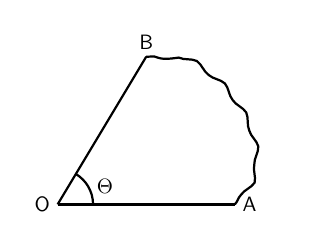
\begin{tikzpicture}[thick,scale=0.75, every node/.style={scale=0.75}]
    % Coordinates of the triangle vertices
    \coordinate[label=left:O] (O) at (0,0);
    \coordinate[label=right:A] (A) at (3,0);
    \coordinate[label=above:B] (B) at (1.5,2.5);

    % Drawing the triangle
    \draw (O) -- (A);
    \draw (O) -- (B);
    % Labeling the angle
    \draw (0.6,0) arc (0:60:0.6);
    \node at (0.8,0.3) {$\Theta$};
    \draw [decorate, decoration={snake, amplitude=0.3mm, segment length=4.5mm}] (A) to[out=45, in=0] (B);
\end{tikzpicture}
\caption{A wedge-like ``shape'' with an interior angle \(\Theta\).}\label{wedge}
\end{figure}

To incorporate the singular behavior near a corner with less regularity and (possible) singularities, first assume, without loss of generality, that the domain \(\Omega\) has just one corner and that the solution of our BVP can be decomposed in regular and singular parts,
\[
    u(x) = u_R(x) + u_S(x), \; x \in \overline{\Omega},
\]
where \(u_R\) is the regular part approximated by the MFS basis functions and the singular part \(u_S\) is approximated by Fourier expansions using the families of particular solutions \eqref{particular_sol_with_alpha} and \eqref{particular_sol_without_alpha}, having the boundary conditions into account. Let \(\phi_s(r, \theta)\) be one of those expansions centered at the corner's tip, where \(s\) is the order of the expansion. Then, the numerical approximation can be written as
\begin{equation}\label{expansion_particular}
    \tilde{u}(x) = \sum_{j=1}^{N}\alpha_j \Phi(x-y_j) + \alpha_{N+1} + \sum_{s=1}^{P} \beta_s \phi_s(r(x),\theta(x)), \; x \in \overline{\Omega},
\end{equation}
where \(P\) is the order of the expansion in particular solutions, the matrix \(A\) and the vector \(\alpha\) in \eqref{MFS_m_system} are adjusted accordingly using equation \eqref{expansion_particular}.

For the Helmholtz equation, the approach is almost the same, although one must also compute the \sloppy eigenvalues/eigenfrequencies of the differential operator \(\mathcal{L} = -(\Delta + k^2)\). For example, if considering Dirichlet boundary conditions, Theorem \ref{MFS_helm_null_kern} below gives a way to search for them.
\begin{theorem}\label{MFS_helm_null_kern}
    If \(k\) is not an eigenfrequency of the interior Dirichlet problem, then \(\dim \left(\ker(S_k)\right)=0\), where
    \[
    S_k \varphi(y) = \int_{\hat{\Gamma}}\Phi(x-y)_k\varphi(y)d\sigma(y).
    \]
\end{theorem}

In practice, one obtains a system of equations analogous to the system \eqref{MFS_m_system}, which now depends on some value \(k\). By Theorem \ref{MFS_helm_null_kern}, an eigenfunction \(u\) associated with an eigenfrequency \(k\) of the Laplace operator in an element of the kernel of \(S_k\), i.e. \(u \in \ker(S_k)\). Thus, we look for a matrix \(A\) in \eqref{MFS_m_system} such that its kernel is not trivial. If \(A\) is a squared matrix, this can be done by computing its determinant; otherwise, one can compute its smallest singular value \(\sigma_N\). In this work, we also used the Subspace Angle Technique introduced in \cite{betcke2005reviving} in order to reduce the condition number \(k(A)\) of matrix \(A\).

\section{Numerical Results}

\subsection{Dirac equation simulations}

In this section, we briefly summarize our findings for the Dirac operator with infinite mass boundary conditions. The Helmholtz equation with Cauchy-Riemman oblique boundary conditions \eqref{helm_system} was used for the Dirac operator. First, we address Conjecture \ref{david_conjectures}, which is corroborated by Figures \ref{eigenvalues_rectangle_width_m_1} and \ref{eigenvalues_rectangle_width_m_5}. Several
interesting observations can be made:
\begin{enumerate}
    \item \label{dirac_sim_quad_point_1} the eigenvalues for varying \(m\) approach \(m\) with a diminishing gap, remaining above \(m\). From Figure \ref{eigenvalues_rectangle_width_m_1} it is possible to see that the global minimizer of the third eigenvalue is not a square for \(m=1\), but for a certain rectangle with width \(a \approx 2.2\). We point out that the square is indeed the minimizer of the third eigenvalue for any mass \(m\) above some critical mass \(1 \leq m_{\text{crit}} \leq 5\);

    \item \label{dirac_sim_quad_point_2} starting from the third eigenvalue, spikes appear, indicating eigenvalues with multiplicity 2, such as the third and fourth eigenvalues coinciding between 1 and 1.5. This multiplicity pattern becomes more frequent as the order of the eigenvalues increases;

    \item \label{dirac_sim_quad_point_3} increasing \(a\) causes linear growth in eigenvalue magnitude without altering multiplicity. As \(a\) grows, eigenvalues converge due to the transformation of the domain into an unbounded line, resulting in a continuous spectrum.
\end{enumerate}
\begin{figure}
    \centering
    \begin{minipage}{.25\textwidth}
      \centering
      \includegraphics[width=\linewidth]{/home/francisco/Universidade/Tese/Report/Report/Images/Dirac/quad/eigenvalues_rectangle_width_m_1.png}
      \captionsetup{width=0.9\linewidth} % Adjust the width of the caption
      \captionof{figure}{Behavior of the first five eigenvalues for rectangles with unit area, width \(a\) and \(m=1\).}
      \label{eigenvalues_rectangle_width_m_1}
    \end{minipage}%
    %\hspace{0.5cm} % Add some horizontal space between the figures
    \begin{minipage}{.25\textwidth}
      \centering
      \includegraphics[width=1\linewidth]{/home/francisco/Universidade/Tese/Report/Report/Images/Dirac/quad/eigenvalues_rectangle_width_m_5.png}
      \captionsetup{width=0.9\linewidth} % Adjust the width of the caption
      \captionof{figure}{Behavior of the first five eigenvalues for rectangles with unit area, width \(a\) and \(m=5\).}
      \label{eigenvalues_rectangle_width_m_5}
    \end{minipage}
\end{figure}

Analogously, Figures \ref{eigenvalues_rectangle_perimeter_width_m_1} and \ref{eigenvalues_rectangle_perimeter_width_m_5} are in line with the Conjecture \ref{david_conjectures}. The conclusions and remarks presented in points \ref{dirac_sim_quad_point_1} and \ref{dirac_sim_quad_point_2} for rectangles with fixed area are still valid. In this case, point \ref{dirac_sim_quad_point_3} holds when \(a\) approaches zero.
\begin{figure}
    \centering
    \begin{minipage}{.25\textwidth}
      \centering
      \includegraphics[width=\linewidth]{/home/francisco/Universidade/Tese/Report/Report/Images/Dirac/quad/eigenvalues_rectangle_perimeter_width_m_1.png}
      \captionsetup{width=0.9\linewidth} % Adjust the width of the caption
      \captionof{figure}{Behavior of the first five eigenvalues for rectangles with perimeter \(L=4\), width \(a\) and \(m=1\).}
      \label{eigenvalues_rectangle_perimeter_width_m_1}
    \end{minipage}%
    %\hspace{0.5cm} % Add some horizontal space between the figures
    \begin{minipage}{.25\textwidth}
      \centering
      \includegraphics[width=1\linewidth]{/home/francisco/Universidade/Tese/Report/Report/Images/Dirac/quad/eigenvalues_rectangle_perimeter_width_m_5.png}
      \captionsetup{width=0.9\linewidth} % Adjust the width of the caption
      \captionof{figure}{Behavior of the first five eigenvalues for rectangles with perimeter \(L=4\), width \(a\) and \(m=5\).}
      \label{eigenvalues_rectangle_perimeter_width_m_5}
    \end{minipage}
\end{figure}

Simulations were conducted for general quadrilaterals with \(m=1\) and are presented in Figure \ref{dirac_first_three_eigenvalues_quad_m_1}. This includes rectangles and rhombi, where Conjecture \ref{david_conjectures} generally seems to be confirmed. Surprisingly, our simulations reveal that, for \(m=1\), the domain that minimizes the third eigenvalue is not the unit disk. This contradicts expectations, as it is conjectured to be the case for the Dirichlet Laplacian problem. This observation underscores the influence of the mass (\(m\)) of the relativistic particle on the Dirac operator's spectrum. Furthermore, our simulations validate Conjecture \ref{conjecture_benguria}, as demonstrated in Figure \ref{dirac_benguria_quad}.
\begin{figure}[h]
    \begin{minipage}[t]{0.4\textwidth}
        \centering
        \includegraphics[width=1.1\textwidth]{/home/francisco/Universidade/Tese/Report/Report/Images/Dirac/quad/first_three_eigenvalues_quad_m_1.png}
        \caption{Plot of the first three eigenvalues against the perimeter for \(m=1\) for quadrilaterals. The ``outliers'' marked in black represent the domains in which the third eigenvalue is smaller than the third eigenvalue of the disk.}
        \label{dirac_first_three_eigenvalues_quad_m_1}
    \end{minipage}
    \hfill
    \hspace{0.5cm}
    \begin{minipage}[t]{0.4\textwidth}
        \centering
        \includegraphics[width=0.7\textwidth]{/home/francisco/Universidade/Tese/Report/Report/Images/Dirac/quad/benguria_quad.png}
        \captionsetup{width=0.65\linewidth} % Adjust the width of the caption
        \caption{Ratio between the first two eigenvalues \(\frac{\lambda_2}{\lambda_1}\) plotted against the perimeter for \(m=1\) for quadrilaterals, as in Figure \ref{dirac_first_three_eigenvalues_quad_m_1}.}
        \label{dirac_benguria_quad}
    \end{minipage}
\end{figure}

For triangles, we systematically address Conjectures \ref{triangle_conjectures} for \(m=1\). An admissible triangle \(T\) is defined within region \(R\) with piecewise boundary \(\partial R = \Gamma_0 \cup \Gamma_1 \cup \Gamma_2\), where
\[
    R = \{(x, y) \in \mathbb{R}^2: x \geq 0, y > 0, (x+1)^2 + y^2 \leq 4\}.
\]
A triangle \(T\) is subequilateral if its basis vertices are \((0, 0)\) and \((1, 0)\) with a third vertex \((x, y)\) in \(\Gamma_1\) and superequilateral if in \(\Gamma_2\), being equilateral at \((0, \sqrt{3})\). This systematic approach exhausts all possible triangles up to congruence within region \(R\). For brevity, we present results for fixed unit area, but it is important to note that similar results for the perimeter also support Conjecture \ref{triangle_conjectures}. Figure \ref{dirac_smooth_first_eigenvalue} resembles Figure \ref{dirac_first_three_eigenvalues_quad_m_1} for quadrilaterals but focuses solely on the first eigenvalue. Given our systematic approach, which explores all types of triangles up to congruence, and the eigenvalues are continuous with respect to domain perturbations, it is improbable that the conjectures for triangles (especially for \(m=1\)) do not hold. Once again, Figure \ref{dirac_triangle_benguria} suggests that Conjecture \ref{conjecture_benguria} holds.
\begin{figure}[h]
    \centering
    \begin{minipage}{.25\textwidth}
      \centering
      \includegraphics[width=\textwidth]{/home/francisco/Universidade/Tese/Report/Report/Images/Dirac/triangles/triangle_first_eigenvalue.png}
      \captionsetup{width=0.9\linewidth} % Adjust the width of the caption
      \captionof{figure}{Plot of the first eigenvalue against the perimeter for triangular domains.}
    \label{dirac_smooth_first_eigenvalue}
\end{minipage}%
    %\hspace{0.5cm} % Add some horizontal space between the figures
    \begin{minipage}{.25\textwidth}
      \centering
      \includegraphics[width=\textwidth]{/home/francisco/Universidade/Tese/Report/Report/Images/Dirac/triangles/triangle_benguria.png}
      \captionsetup{width=0.9\linewidth} % Adjust the width of the caption
      \captionof{figure}{Ratio between the first two eigenvalues \(\frac{\lambda_2}{\lambda_1}\) for triangular domains.}
    \label{dirac_triangle_benguria}
\end{minipage}
\end{figure}

For polygonal domains, our simulations were less intensive and we only present our results for Conjecture \ref{polya_szego_conjecture_dirac}, for polygons with fixed area and \(m=1\) in Figures \ref{dirac_polya_szego_evidence_pentagons}, \ref{dirac_polya_szego_evidence_hexagons}, \ref{dirac_polya_szego_evidence_heptagons} and \ref{dirac_polya_szego_evidence_octagons}. As expected, the Conjecture appears to hold for \(n\)-sided polygons with \(n=5,6,7,8\) and \(m=1\).
\begin{figure}
    \centering
    \begin{minipage}[b]{0.2\textwidth}
        \centering
        \includegraphics[width=\textwidth]{/home/francisco/Universidade/Tese/Report/Report/Images/Dirac/Polygons/pentagons.png}
    \caption{Numerical simulations in the first eigenvalue of general pentagons.}
    \label{dirac_polya_szego_evidence_pentagons}
    \end{minipage}
    \hfill
    \begin{minipage}[b]{0.2\textwidth}
        \centering
        \includegraphics[width=\textwidth]{/home/francisco/Universidade/Tese/Report/Report/Images/Dirac/Polygons/hexagons.png}
    \caption{Numerical simulations in the first eigenvalue of general hexagons.}
    \label{dirac_polya_szego_evidence_hexagons}
    \end{minipage}

    \vspace{0.5cm}

    \begin{minipage}[b]{0.2\textwidth}
        \centering
        \includegraphics[width=\textwidth]{/home/francisco/Universidade/Tese/Report/Report/Images/Dirac/Polygons/heptagons.png}
    \caption{Numerical simulations in the first eigenvalue of general heptagons.}
    \label{dirac_polya_szego_evidence_heptagons}
    \end{minipage}
    \hfill
    \begin{minipage}[b]{0.2\textwidth}
        \centering
        \includegraphics[width=\textwidth]{/home/francisco/Universidade/Tese/Report/Report/Images/Dirac/Polygons/octagons.png}
    \caption{Numerical simulations in the first eigenvalue of general octagons.}
    \label{dirac_polya_szego_evidence_octagons}
    \end{minipage}
\end{figure}
In our final set of simulations for the Dirac operator, we maintained $m=1$ as a fixed parameter and focused on smooth domains. This choice offered two advantages: first, it allowed for a wide range of arbitrary domain shapes, enhancing the reliability of numerical approximations. Second, it enabled the exploration of the domain that minimizes the third eigenvalue. To generate random smooth domains, we employed periodic B-spline interpolation \cite{de1978practical} in each vector component. Since our simulations for smooth domains are in line with the previous results, here we only address the (global) minimization of the third eigenvalue for fixed area, as we already know that there exists some domain whose third eigenvalue is smaller than that of the disk.

Let $\mathcal{F}(\Omega) = \lambda_3(\Omega)$ be the functional which maps each smooth domain $\Omega$ to its corresponding third eigenvalue, and $\Omega_0$ be the detected domain with the smallest third eigenvalue. We consider the constrained minimization problem
\begin{equation}
    \min_{\substack{\Omega \subset \mathbb{R}^2 \\ \abs{\Omega}=1}} \mathcal{F}(\Omega).
\end{equation}

Since no (shape) derivative is known for the eigenvalues of the Dirac operator with infinite mass boundary conditions, we resorted to the Nelder-Mead algorithm, a direct optimization method in high-dimensional spaces. We considered a polar approximation of $\Omega$ given by the Fourier expansion
\begin{equation}
    r(\theta_i) \approx a_0 + \sum_{m=1}^{M}a_m \cos(m \theta_i) + \sum_{m=1}^{M}b_m \sin(m \theta_i),
\end{equation}
where $M$ is the order of the trigonometric interpolation, $\theta_i$ is a collocation point on the domain $\Omega$ for $i=1,\dots,N$, and $a_0,\dots, a_m,\dots, b_m,\dots,b_M$ are the coefficients found through least squares. Therefore, we transform equation (1) into a discrete optimization problem in $\mathbb{R}^{2M+1}$. Iteratively, and always normalizing the domain into unit area, we use the Nelder-Mead algorithm to find the optimal shape that minimizes the third eigenvalue with $m=1$. The results are presented in Figure \ref{dirac_nelder_mead_domain}. Since the eigenvalues are continuous with respect to domain perturbations, Figure \ref{dirac_val_third} presents the results of a Minkowski sum, validating our findings.
\begin{figure}
    \centering
    \begin{minipage}{.26\textwidth}
        \centering
        \includegraphics[width=0.9\linewidth]{/home/francisco/Universidade/Tese/Report/Report/Images/Dirac/smooth/nelder_mead_optimal.png}
        \captionsetup{width=0.8\linewidth} % Adjust the width of the caption
        \captionof{figure}{Optimal domain \(\Omega^\star\) (drawn in orange) and the initial domain (in blue) used in the first iteration of the Nelder-Mead algorithm.}
        \label{dirac_nelder_mead_domain}
    \end{minipage}%
    %\hspace{0.5cm} % Add some horizontal space between the figures
    \begin{minipage}{.26\textwidth}
        \centering
        \includegraphics[width=0.8\linewidth]{/home/francisco/Universidade/Tese/Report/Report/Images/Dirac/smooth/dirac_val_third.png}
        \captionsetup{width=0.8\linewidth} % Adjust the width of the caption
        \captionof{figure}{The first three eigenvalues in domains defined by the Minkowski sum \(\Omega_t\) and plotted for the values of \(t\in [0,1]\) increasing from left to right.}
        \label{dirac_val_third}
    \end{minipage}
\end{figure}

\subsection{Transmission problem}

In this section, we summarize our findings for the decomposition problem with transmission conditions. The procedure presented here is based on \cite{alves2005new} and \cite{alves2021domain}. As in \cite{gustafsson2019error}, we take the source functions \(f_i = 1, \, i=1, 2\). In this case, a solution of \eqref{decomp_prob} can be found by taking the following steps:
\begin{enumerate}
    \item \label{chapter_numerics_t_p_particular_prodecure} find a non-homogeneous solution for the non-homogeneous problem
    \[
        \begin{cases}
            -\Delta u_1^{NH} = \frac{1}{k_1}\\
            -\Delta u_2^{NH} = \frac{1}{k_2},
        \end{cases}
    \]
    in \(\mathbb{R}^2\) which does not necessarily satisfy the boundary and interface conditions in \eqref{decomp_prob}. This can easily be done, and
    \[
        \begin{cases}
            u_1^{NH} = -\frac{x_1^2 + x_2^2}{4k_1}\\
            u_2^{NH} = -\frac{x_1^2 + x_2^2}{4k_2}
        \end{cases}
    \]
    are some possible non-homogeneous solutions;
    \item then we solve the homogeneous problem
    \begin{align}\label{transmission_num_homo}
        \begin{cases}
        - \Delta u_i^H = 0, & \text{in }\Omega_i\\
        u_1^H - u_2^H = u_2^{NH}- u_1^{NH}, & \text{on }\gamma\\
        k_1 \frac{\partial u_1^H}{\partial \mathbf{n_1}} - k_2 \frac{\partial u_2^H}{\partial  \mathbf{n_1}} = k_2 \frac{\partial u_2^{NH}}{\partial  \mathbf{n_1}}  - k_1 \frac{\partial u_1^{NH}}{\partial  \mathbf{n_1}}, & \text{on }\gamma\\
        u_i^H = - u_i^{NH}, & \text{on }\Gamma_i,
        \end{cases}
    \end{align}
    for \(u_1^H\) and \(u_2^H\);
    \item finally, the solution of \eqref{decomp_prob} is \(u_i = u_i^H + u_i^{NH}\).
\end{enumerate}

Let \(N^{(i)}\) denote the number of source points at each domain and \(N=N^{(1)}+N^{(2)}\). We denote the approximate solution by
\[
    \tilde{u} = \begin{cases}
        \tilde{u}_1, & \text{in } \Omega_1\\
        \tilde{u}_2, & \text{in } \Omega_2,
    \end{cases}
\]
where
\begin{align*}
    &\tilde{u}_1(x) = \sum_{j=1}^{N^{(1)}} \alpha^{(1)}_j \Phi\left(x-y_j^{(1)}\right)\\
    &\tilde{u}_2(x) = \sum_{j=1}^{N^{(2)}} \alpha^{(2)}_j \Phi\left(x-y_j^{(1)}\right).
\end{align*}
Let \(M^{(i)}\) be the number of boundary collocation points \(x^{(i)}_{m}\) for each \(\Omega_i\) and \(M=M^{(1)}+M^{(2)}\). We also consider \(Q\) interface points \(z_q \in \gamma\) with \(q=1,\dots,Q\). Then, we arrive to a block system similar to \eqref{MFS_m_system}, where the matrix \(A\) is given by
\footnotesize\begin{equation*}
    A = \begin{bmatrix}
        \left[\Phi\left(x^{(1)}_{m}-y_j^{(1)}\right)\right]_{M^{(1)}\times N^{(1)}} & [0]_{M^{(1)}\times N^{(2)}} \\
        [0]_{M^{(2)}\times N^{(1)}} & \left[\Phi\left(x^{(2)}_{m}-y_j^{(2)}\right)\right]_{M^{(2)}\times N^{(2)}} \\
        \left[\Phi\left(z_q-y_j^{(1)}\right)\right]_{Q\times N^{(1)}} & \left[-\Phi\left(z_q-y_j^{(2)}\right)\right]_{Q\times N^{(2)}} \\
        \left[k_1\partial_n \Phi\left(z_q-y_j^{(1)}\right)\right]_{Q\times N^{(1)}} & \left[-k_2 \partial_n \Phi\left(z_q-y_j^{(2)}\right)\right]_{Q\times N^{(2)}}
    \end{bmatrix},
\end{equation*}\normalsize
whose dimensions are \((M^{(1)}+M^{(2)}+2Q)\times(N^{(1)}+N^{(2)})\), and the vector \(b\) is of the form
\footnotesize \begin{equation*}
        b = \begin{bmatrix}
        \left[-u_1^{NH}(x^{(1)}_{m})\right]_{M^{(1)}\times 1}\\
        \left[-u_2^{NH}(x^{(2)}_{m})\right]_{M^{(2)}\times 1}\\
        \left[u_2^{NH}(z_q)-u_1^{NH}(z_q)\right]_{Q\times 1}\\
        \left[k_2 \partial_n u_2^{NH}(z_q)- k_1 \partial_n u_1^{NH}(z_q)\right]_{Q\times 1}\\
    \end{bmatrix}.
\end{equation*}\normalsize

Given the complexity of the problems at hand, closed-form solutions are not available, and we can only check for consistency errors which measure how accurately the interface and boundary conditions are satisfied:
\begin{itemize}
    \item \(\norm*{\tilde{u}_i - 0}_{L^2(\Gamma_i)}\), \(i=1, 2\): boundary collocation error;
    \item \(e_\gamma^0 = \norm*{\tilde{u}_1 - \tilde{u}_2}_{L^2(\gamma)}\), \(i=1, 2\): \(L^2\) error of \(\tilde{u}\) across \(\gamma\);
    \item \(e_\gamma^1 = \norm*{k_1 \partial_n\tilde{u}_1 - k_2 \partial_n\tilde{u}_2}_{L^2(\gamma)}\), \(i=1, 2\): \(L^2\) error of \(\partial_n\tilde{u}\) across \(\gamma\).
\end{itemize}
From a numerical point of view, let \(\mathcal{I}\) be the sample of test points. The \(L^2\) norm is discretized into the Root Mean Squared Error (RMSE) which is equivalent to the \(l^2\) norm and is given by
\[
    \norm*{u-\tilde{u}}= \sqrt{\frac{1}{\#\mathcal{I}} \sum_{z \in \mathcal{I}} \abs{u(z)-\tilde{u}(z)}^2}.
\]
For every result, we fixed \(k_2=1\) since the ratio \(\frac{k_1}{k_2}\) is responsible for the behavior of the solutions near the interface.

For the sake of brevity, we focus on a rectangular domain \([-1, -0.5] \times [1, 0.5]\) with a vertical interface along the line \(x=0\). We aim to study the problem for \(k_1 \neq k_2\), where \(k_2=1\) is fixed. The results presented in Table \ref{tab:transmission_results_rectangle} for each value of \(k\) were obtained using 600 boundary points and 404 source points in each domain.
\begin{table}
    \centering
    \footnotesize % Reduce the font size
    \setlength{\tabcolsep}{1pt} % Reduce the column spacing
    \begin{tabular}{@{}cccccc@{}}
      \toprule
      \multirow{2}{*}{\textbf{\(k_1\) value}} & \multicolumn{2}{c}{\textbf{Boundary Error}} & \multicolumn{2}{c}{\textbf{Interface Errors}} \\
      \cmidrule(lr){2-3} \cmidrule(lr){4-5}
      & \textbf{Domain 1} & \textbf{Domain 2} & \textbf{\(e_\gamma^0\)} & \textbf{\(e_\gamma^1\)} & \\
      \midrule
      1 & $7.775\times10^{-8}$ & $7.779\times10^{-8}$ & $4.732\times10^{-9}$ & $7.589\times10^{-9}$\\
      2 & $4.398\times10^{-8}$ & $8.614\times10^{-8}$ & $2.499\times10^{-6}$ & $7.868\times10^{-8}$\\
      5 & $2.181\times10^{-8}$ & $1.036\times10^{-7}$ & $3.838\times10^{-6}$ & $1.551\times10^{-7}$\\
      \bottomrule
    \end{tabular}
    \caption{Consistency errors on the boundary and at the interface \(\gamma\).}
    \label{tab:transmission_results_rectangle}
\end{table}
\begin{figure}
    \centering
    \begin{minipage}{.25\textwidth}
      \centering
      \includegraphics[width=\linewidth]{/home/francisco/Universidade/Tese/Report/Report/Images/Transmission/Rectangle_contour_600_150_k1_1.png}
      \captionsetup{width=0.8\linewidth} % Adjust the width of the caption
      \captionof{figure}{Numerical simulation with  \(k_1=1\).}
      \label{transmission_rectangle_plot_k1_1}
    \end{minipage}%
    \begin{minipage}{.25\textwidth}
      \centering
      \includegraphics[width=\linewidth]{/home/francisco/Universidade/Tese/Report/Report/Images/Transmission/Rectangle_contour_600_150_k1_2.png}
      \captionsetup{width=0.8\linewidth} % Adjust the width of the
      \captionof{figure}{Numerical simulation with \(k_1=2\).}
      \label{transmission_rectangle_plot_k1_2}
    \end{minipage}
    \caption*{Numerical approximations of the BVP for a rectangular domain with different \(k_1\) values.}
    \label{transmission_rectangle_plots}
\end{figure}

Notice that as \(k_1\) increases, the symmetry of the solution is disrupted, causing a shift from \(\Omega_1\) (the left domain) to \(\Omega_2\) (the right domain). Note that these results are dependent on the domain, and lose accuracy due to reduced domain regularity, although a high level of accuracy is achieved for rectangles. It is worth mentioning that when \(k_1\) and \(k_2\) have different values, the method's accuracy decreases, as expected, since the material parameter changes at the interface, reducing the solution's regularity.

In the context of the rectangular problem, we chose not to expand our set of basis functions, as the traditional basis functions used in the MFS captured the solution's behavior around the corners due to their alignment with the right angles. In what follows we consider the case of an L-shaped, nonconvex domain whose solutions are less regular due to the re-entrant corner. Two different interfaces will be considered: first, the interface along the line \(x=0\); then, along the symmetry axis of the domain \(\Omega\), i.e. along the line \(y=x+\frac{1}{2}\).

For the first case with the interface along the line \(x=0\), there are 300 interface points, and each domain has 428 source points. The number of boundary collocation points for \(\Omega_1\) and \(\Omega_2\) is 710 and 639, respectively. In Figure \ref{transmission_L_shape_k1_5}, \(\Omega_1\) represents the domain on the left of the interface, and \(\Omega_2\) is on the right.
\begin{figure}
    \centering
    \includegraphics[width=0.65\linewidth]{/home/francisco/Universidade/Tese/Report/Report/Images/Transmission/L_shape_2_rectangles_k1_5.png}
    \captionsetup{width=\linewidth} % Adjust the width of the caption
    \caption{Numerical approximation of the transmission problem in an L-shaped domain with interface along \(x=0\) and \(k_1=5\).}
    \label{transmission_L_shape_k1_5}
\end{figure}

In Table \ref{tab:transmission_results_L_shape_rectangles}, results without enrichment techniques reveal reduced accuracy, primarily due to the solution's lower regularity near the re-entrant corner. The interface error, notably its discontinuity, increases, even with increased interface collocation points. This suggests that domain geometry presents greater challenges than the discontinuous source function, particularly with varying material parameters \(k_1\) and \(k_2\). Figure \ref{transmission_L_shape_k1_5} illustrates this complexity with a small jump near the interface edges.
\begin{table}
    \centering
    \footnotesize % Reduce the font size
    \setlength{\tabcolsep}{1pt} % Reduce the column spacing
    \begin{tabular}{@{}cccccc@{}}
      \toprule
      \multirow{2}{*}{\textbf{\(k_1\) value}} & \multicolumn{2}{c}{\textbf{Boundary Error}} & \multicolumn{2}{c}{\textbf{Interface Errors}} \\
      \cmidrule(lr){2-3} \cmidrule(lr){4-5}
      & \textbf{Domain 1} & \textbf{Domain 2} & \textbf{\(e_\gamma^0\)} & \textbf{\(e_\gamma^1\)} & \\
      \midrule
      1 & $7.853\times10^{-5}$ & $1.155\times10^{-4}$ & $2.916\times10^{-3}$ & $2.155\times10^{-5}$ \\
      2 & $8.152\times10^{-5}$ & $1.350\times10^{-4}$ & $3.835\times10^{-3}$ & $1.149\times10^{-5}$\\
      5 & $7.079\times10^{-5}$ & $1.378\times10^{-4}$ & $4.085\times10^{-3}$ & $5.411\times10^{-5}$\\
      \bottomrule
    \end{tabular}
    \caption{Consistency errors on the boundary and in the interface \(\gamma\)}
    \label{tab:transmission_results_L_shape_rectangles}
\end{table}
For basis functions enrichment, we consider Dirichlet-Neumann particular solutions centered in the singular corner for \(\Omega_1\). Notice that for \(\Omega_2\) these types of particular solutions are not added to the set of basis functions since the interface edges make a right angle with the adjacent edges.
Therefore, we only consider particular solutions that describe the behavior of the solution in the \(\pi\) radians corner with a possible singularity. Let
\begin{equation}
    v_{p_1}(r, \theta) = \beta_{p_1} r^{\alpha_{p_1}} \sin(\beta_{p_1}(\theta - \theta_1))
\end{equation}
where
\begin{equation}\label{dir_neumman_betas}
    \beta_{p_1} = \frac{(p_1+\frac{1}{2})\pi}{\Theta},
\end{equation}
\(\theta_1 = \frac{\pi}{2}\) and \(\Theta = \pi\) is the total angle amplitude. Finally, considering the truncated expansion
\begin{equation}\label{num_particular_L_shape_rect_equation}
    \phi(r,\theta)=\sum_{p_1=0}^{P_1} \delta_{p_1} v_{p_1}(r, \theta),
\end{equation}
where \(P_1\) is the number of particular solutions added and \(\{\delta_{p_1}\}_{p_1=1,\dots,P_1}\) the coefficients to be found using least squares.

Table \ref{tab:transmission_results_L_shape_rectangles_particular} presents results after applying enrichment techniques for various \(k_1\) values. In equation \eqref{num_particular_L_shape_rect_equation}, different term counts were examined. For positive \(p_1\) values, increasing \(P_1\) beyond 2 did not improve results. Surprisingly, introducing particular solutions for the exterior problem led to reduced errors along the domain boundaries \(\Gamma_i\) and improved interface results.
\begin{table}
    \centering
    \footnotesize % Reduce the font size
    \setlength{\tabcolsep}{1pt} % Reduce the column spacing
    \begin{tabular}{cccccc}
        \toprule
        \multicolumn{1}{c}{\textbf{\(p_1\) values}} & \multicolumn{1}{c}{\textbf{\(k_1\) value}} & \multicolumn{2}{c}{\textbf{Boundary Error}} & \multicolumn{2}{c}{\textbf{Interface Errors}} \\
        \cmidrule(lr){2-2} \cmidrule(lr){3-4} \cmidrule(lr){5-6}
        & & \textbf{Domain 1} & \textbf{Domain 2} & \textbf{\(e_\gamma^0\)} & \textbf{\(e_\gamma^1\)} \\
        \midrule

        % Data for p = [0, 1]
        0, 1 & 1 & $2.965\times10^{-5}$ & $7.907\times10^{-5}$ & $2.94\times10^{-3}$ & $2.624\times10^{-5}$ \\
        & 2 & $2.203\times10^{-5}$ & $6.657\times10^{-5}$ & $1.86\times10^{-3}$ & $2.068\times10^{-5}$ \\
        & 5 & $2.203\times10^{-5}$ & $6.657\times10^{-5}$ & $1.86\times10^{-3}$ & $2.068\times10^{-5}$ \\
        \midrule

        % Data for p = [-1, 0, 1]
        -1, 0, 1 & 1 & $8.627\times10^{-6}$ & $4.132\times10^{-5}$ & $7.68\times10^{-4}$ & $6.876\times10^{-6}$ \\
        & 2 & $7.333\times10^{-6}$ & $2.791\times10^{-5}$ & $6.01\times10^{-4}$ & $2.555\times10^{-5}$ \\
        & 5 & $4.271\times10^{-6}$ & $1.118\times10^{-5}$ & $2.69\times10^{-4}$ & $4.166\times10^{-5}$ \\
        \midrule

        % Data for p = [-2, -1, 0, 1]
        -2, -1, 0, 1 & 1 & $3.898\times10^{-6}$ & $5.975\times10^{-6}$ & $1.44\times10^{-3}$ & $2.505\times10^{-6}$ \\
        & 2 & $2.584\times10^{-6}$ & $2.514\times10^{-6}$ & $9.69\times10^{-4}$ & $1.048\times10^{-5}$ \\
        & 5 & $1.119\times10^{-6}$ & $6.838\times10^{-7}$ & $4.89\times10^{-4}$ & $1.106\times10^{-5}$ \\
        \bottomrule
    \end{tabular}
    \caption{Consistency errors on the boundary and at the interface \(\gamma\) after enriching the basis with particular (angular) solutions}
    \label{tab:transmission_results_L_shape_rectangles_particular}
\end{table}

To finish the study of the domain decomposition problem with transmission conditions and basis enrichment, we investigate an L-shaped domain with the interface aligned along its axis of symmetry. This configuration features two singular corners, each with an angle of \(\frac{3}{4}\pi\) radians, while the other two corners have angles of \(\frac{\pi}{4}\) radians, which do not pose challenges for classical MFS basis functions. Each domain includes 300 interface points, 428 source points, and 628 boundary collocation points. Table \ref{tab:transmission_results_L_shape_axis} provides a summary of the results obtained without the use of particular solutions.

\begin{table}
    \centering
    \footnotesize % Reduce the font size
    \setlength{\tabcolsep}{1pt} % Reduce the column spacing
    \begin{tabular}{cccccc}
        \toprule
        \multirow{2}{*}{\textbf{\(k_1\) value}} & \multicolumn{2}{c}{\textbf{Boundary Error}} & \multicolumn{2}{c}{\textbf{Interface Errors}} \\
        \cmidrule(lr){2-3} \cmidrule(lr){4-5}
        & \textbf{Domain 1} & \textbf{Domain 2} & \textbf{\(e_\gamma^0\)} & \textbf{\(e_\gamma^1\)} \\
        \midrule
        1 & $1.812\times10^{-4}$ & $2.060\times10^{-4}$ & $7.305\times10^{-3}$ & $8.018\times10^{-5}$ \\
        2 & $1.398\times10^{-4}$ & $9.729\times10^{-5}$ & $5.986\times10^{-4}$ & $5.505\times10^{-5}$ \\
        5 & $7.096\times10^{-5}$ & $3.030\times10^{-5}$ & $1.528\times10^{-3}$ & $4.348\times10^{-5}$ \\
        \bottomrule
    \end{tabular}
    \caption{Consistency errors on the boundary and at the interface \(\gamma\).}
    \label{tab:transmission_results_L_shape_axis}
\end{table}

For the domain \(\Omega_2\), one can now consider the incorporation of Neumann-Dirichlet particular solutions centered at the corner which imposes less regularity on the solution. These particular solutions are of the form
\[
w_{p_2}(r,\theta) = \beta_{p_2} r^{\beta_{p_2}}\cos(\beta_{p_2}(\theta-\theta_2)),
\]
where the coefficients \(\beta_{p_2}\) mirror\footnote{By making the straightforward transition from \(p_1\) to \(p_2\).} those in \eqref{dir_neumman_betas}, \(\theta_2=\frac{5}{4}\pi\) and while \(\Theta = \frac{3}{4}\pi\) remains consistent across both domains.
\begin{table}[!htbp]
    \centering
    \footnotesize % Reduce the font size
    \setlength{\tabcolsep}{1pt} % Reduce the column spacing
    \begin{tabular}{cccccc}
        \toprule
        \multicolumn{1}{c}{\textbf{\(p_1\) values}} & \multicolumn{1}{c}{\textbf{\(k_1\) value}} & \multicolumn{2}{c}{\textbf{Boundary Error}} & \multicolumn{2}{c}{\textbf{Interface Errors}} \\
        \cmidrule(lr){2-2} \cmidrule(lr){3-4} \cmidrule(lr){5-6}
        & & \textbf{Domain 1} & \textbf{Domain 2} & \textbf{\(e_\gamma^0\)} & \textbf{\(e_\gamma^1\)} \\
        \midrule

        % Data for p = [0, 1]
        0, 1 & 1 & $2.965\times10^{-5}$ & $7.907\times10^{-5}$ & $2.94\times10^{-3}$ & $2.624\times10^{-5}$ \\
        & 2 & $2.203\times10^{-5}$ & $6.657\times10^{-5}$ & $1.86\times10^{-3}$ & $2.068\times10^{-5}$ \\
        & 5 & $2.203\times10^{-5}$ & $6.657\times10^{-5}$ & $1.86\times10^{-3}$ & $2.068\times10^{-5}$ \\
        \midrule

        % Data for p = [-1, 0, 1]
        -1, 0, 1 & 1 & $8.627\times10^{-6}$ & $4.132\times10^{-5}$ & $7.68\times10^{-4}$ & $6.876\times10^{-6}$ \\
        & 2 & $7.333\times10^{-6}$ & $2.791\times10^{-5}$ & $6.01\times10^{-4}$ & $2.555\times10^{-5}$ \\
        & 5 & $4.271\times10^{-6}$ & $1.118\times10^{-5}$ & $2.69\times10^{-4}$ & $4.166\times10^{-5}$ \\
        \midrule

        % Data for p = [-2, -1, 0, 1]
        -2, -1, 0, 1 & 1 & $3.898\times10^{-6}$ & $5.975\times10^{-6}$ & $1.44\times10^{-3}$ & $2.505\times10^{-6}$ \\
        & 2 & $2.584\times10^{-6}$ & $2.514\times10^{-6}$ & $9.69\times10^{-4}$ & $1.048\times10^{-5}$ \\
        & 5 & $1.119\times10^{-6}$ & $6.838\times10^{-7}$ & $4.89\times10^{-4}$ & $1.106\times10^{-5}$ \\
        \bottomrule
    \end{tabular}
    \caption{Consistency errors on the boundary and at the interface \(\gamma\) after adding particular (angular) solutions to the classical MFS basis.}
    \label{tab:transmission_results_L_shape_axis_particular}
\end{table}

We observed similar results as before, where negative values for \(p_1\) led to improved approximations, especially when \(k_1 \neq k_2 = 1\). However, we noted that when both \(p_1\) and \(p_2\) were negative, the numerical solution became unstable in both domains and exploded. This suggests that using particular solutions for the exterior problem in both domains is not advisable. On the other hand, when we considered \(p_1 = p_2 = 0, \dots, P\) with \(P > 1\) (e.g., up to \(P = 8\) with 16 particular solutions), our results matched the quality presented in Table \ref{tab:transmission_results_L_shape_axis_particular} for \(p_1=-2, -1, 0, 1\), but only when \(k_1=k_2=1\). Deviating from this condition resulted in a deterioration of the interface approximation. In Figure \ref{transmission_L_axis_plot_k1_2} the numerical approximation is presented.
%, while Figures \ref{transmission_L_axis_error_c0_k1_2} and \ref{transmission_L_axis_error_c1_k1_2} show the absolute error on the interface which peak near the endpoints of the interface, in particular near the re-entrant corner, as expected.
\begin{figure}
    \centering
    \includegraphics[width=0.62\linewidth]{/home/francisco/Universidade/Tese/Report/Report/Images/Transmission/L_shape_2_axis_sol_k1_2_enr.png}
    \caption{Numerical approximation of the transmission problem in an L-shaped domain with interface along the line \(y=x+\frac{1}{2}\) and \(k_1=2\).}
    \label{transmission_L_axis_plot_k1_2}
\end{figure}

\section{Conclusions}

This work explores the Method of Fundamental Solutions in the context of the Dirac operator with infinite mass boundary conditions and transmission problems related to the Poisson equation. It aims to enhance our understanding of the method's capabilities and limitations while presenting its theoretical background.

Regarding the Dirac operator, the extension of the proof concerning the absence of separation of variables in polar coordinates near a corner's tip is numerically significant. Although expected, this extension complicates the use of particular solutions describing angular behavior near a corner. Numerical evidence supports generalizations of the Faber-Krahn inequality and the Ashbaugh-Benguria Theorem for polygonal and smooth domains, enhancing their credibility. Surprisingly, the third eigenvalue's behavior in the Dirac operator's spectrum differs from that of the Laplace operator, particularly at the spectrum's outset, depending on the mass \(m\).

Applying the Method of Fundamental Solutions with particular solutions to transmission problems is significant. This study introduces the novel use of particular solutions to describe the solution's behavior near corners in these PDEs, expanding the method's practical utility.

However, numerous unanswered questions remain, paving the way for future research. Exploring the Dirac operator's spectrum, its distinct behavior compared to the Laplace operator, and optimizing shapes for different eigenvalues are ongoing challenges. Future studies may yield insights into spectral geometry, addressing questions like the optimality of shapes for higher-order eigenvalues. For instance, determining whether the optimal shape for the third eigenvalue is connected remains an unresolved question, potentially leading to revised optimal shape considerations.

The transmission problem using the Method of Fundamental Solutions raises questions and challenges, including the absence of an \textit{a posteriori} error estimate. Exploring alternative particular solutions with improved adaptability to specific problems and enhancing their accuracy at domain interfaces is a potential avenue for refining the Method of Fundamental Solutions, and expanding its utility.

% Our goal is to further this research, address challenges, and extend the methods to advance beyond the current results. This work contributes to refining numerical methods for complex Partial Differential Equations, offering opportunities to gain fresh insights into their behaviors and develop techniques for future research.

% \begin{figure}[!htb]
%     \centering
%     \begin{minipage}{.26\textwidth}
%       \centering
%       \includegraphics[width=1\linewidth]{/home/francisco/Universidade/Tese/Report/Report/Images/Transmission/L_shape_2_axis_c0_error_k1_2_enr.png}
%       \caption{Interface \(\epsilon_\gamma^0\) error}
%       \label{transmission_L_axis_error_c0_k1_2}
%     \end{minipage}%
%     \begin{minipage}{.26\textwidth}
%       \centering
%       \includegraphics[width=1\linewidth]{/home/francisco/Universidade/Tese/Report/Report/Images/Transmission/L_shape_2_axis_c1_error_k1_2_enr.png}
%       \caption{Interface \(\epsilon_\gamma^1\) error}
%       \label{transmission_L_axis_error_c1_k1_2}
%     \end{minipage}
% \end{figure}


{\scriptsize\bibliography{bibliographie.bib}}

\end{document}
